% filename GenericSettings.Rnw 



% filename SimpleGraphs001.Rnw 

%\setcounter{chapter}{} 
\chapter{LURN\ldots{} To Create Simple Graphs} 
\label{SimpleGraphs} 
 
 
 
% filename SimpleGraphs002.Rnw 


% filename SimpleGraphs003.Rnw 


This chapter illustrates the construction of some basic exploratory data analysis graphs. More complex graphs are considered in Chapter~\ref{ComplexGraphs}, although at times we will see graphs presented in conjunction with particular statistical analysis techniques in other chapters. In this chapter, we concentrate on data taking continuous values initially, but a short section on graphs for discrete valued variables is also included. 

There are many ways to create statistical graphs. The traditional method uses one of the base \R{} packages, but in recent years, the \Rpkg{ggplot2} package has gained considerable attention. The presentation of both styles of graph are given throughout this chapter. You will need to ensure the \Rpkg{ggplot2} package is available for use in your \R{} session by issuing the command:
% filename SimpleGraphs004.Rnw 

\begin{Schunk}
\begin{Sinput}
> str(airquality) 
\end{Sinput}
\begin{Soutput}
'data.frame':	153 obs. of  6 variables:
 $ Ozone  : int  41 36 12 18 NA 28 23 19 8 NA ...
 $ Solar.R: int  190 118 149 313 NA NA 299 99 19 194 ...
 $ Wind   : num  7.4 8 12.6 11.5 14.3 14.9 8.6 13.8 20.1 8.6 ...
 $ Temp   : int  67 72 74 62 56 66 65 59 61 69 ...
 $ Month  : int  5 5 5 5 5 5 5 5 5 5 ...
 $ Day    : int  1 2 3 4 5 6 7 8 9 10 ...
\end{Soutput}
\end{Schunk}
% filename SimpleGraphs005.Rnw 

It is common for \R{} users to access the variables after issuing the command 
% filename AttachAirquality.Rnw 

\begin{Schunk}
\begin{Sinput}
> attach(airquality) 
\end{Sinput}
\end{Schunk}
% filename SimpleGraphs007.Rnw 

The \Rcmd{detach} command undoes the \Rcmd{attach} command. To remove the ``attachment", you will issue the command \code{detach(airquality)}. 
 
You could look at the help file for this data if you wanted to learn its complete story using \code{?airquality}. It tells us that the data are for daily readings of the following air quality values for May 1, 1973 (a 
Tuesday) to September 30, 1973. 
\begin{itemize} 
\item \code{Ozone}: Mean ozone in parts per 
billion from 1300 to 1500 hours at Roosevelt Island 
\item \code{Solar.R}: Solar radiation 
in Langleys in the frequency band 4000--7700 Angstroms from 
0800 to 1200 hours at Central Park 
\item \code{Wind}: Average wind speed in miles 
per hour at 0700 and 1000 hours at LaGuardia Airport 
\item \code{Temp}: Maximum daily 
temperature in degrees Fahrenheit at La Guardia Airport. 
\end{itemize} 
 
This data suits our purposes for the majority of examples in this chapter but we will also need to look at another data set for the discussion of graphs for discrete valued variables. 
 
\section{Histograms} 
 
Like many graphical functions in \R{}, the \Rcmd{hist} command will attempt to make a suitably attractive histogram with the minimum of input from the user. Exhibit~\ref{AirQualityHistWind} shows what results from the simplest application of the \Rcmd{hist} command. 
 
Note that the figure created has default settings for the main title, axis labels and that the number of classes (also called bins) and the cutoffs between them have been chosen automatically. Various methods exist for these choices, but it is my recommendation that the user find out what happens when the default settings are chosen and then alter only what is actually necessary. For example, graphs in this document do not always need the default title inserted so we need to suppress the default action if we want to remove the title. We may also want more informative axis labels. Both of these alterations are done for the creation of Exhibit~\ref{AirQualityHistWind2}. \Blind{The need to know what is printed in a histogram was a primary motivator for the development of the BrailleR package and is one of the examples given in Section~\ref{VIExplained} on providing text descriptions of graphs.} 
 
\begin{exhibit} 
\begin{center} 
\caption{Histogram of Average wind speed in miles per hour at 0700 and 1000 hours at LaGuardia Airport. Obtained from the \Robject{air quality} data set.} 
\label{AirQualityHistWind} 
% filename SimpleGraphs008.Rnw 

\begin{Schunk}
\begin{Sinput}
> hist(Wind) 
\end{Sinput}
\end{Schunk}
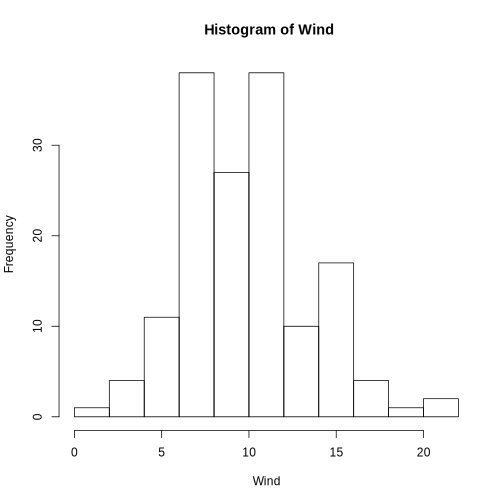
\includegraphics[width=0.8\textwidth,alt={a histogram}]{figures/SimpleGraphsHistAirQualityWind-1} 

\SVGLink{SimpleGraphsHistAirQualityWind} 
% filename SimpleGraphs009.Rnw 

\end{center} 
\end{exhibit} 

\Blind{\subsection*{A note on the visual appearance of the standard histogram for blind users}

A histogram uses rectangles to represent the counts or relative frequencies of observations falling in each subrange of the numeric variable being investigated. The rectangles are standing side by side with their bottom end at the zero mark of the vertical axis. The widths of the rectangles are usually constant, but this can be altered by the user. A sighted person uses the heights and therefore the areas of the rectangles to help determine the overall shape of the distribution, the presence of gaps in the data, and any outliers that might be present. As with most graphs created by the base graphics package, the axes do not join at the bottom left corner and are separated from the area where the data are being plotted. Tick marks are automatically chosen for the data, and the axes may not extend past the ends of variables being plotted. The vertical axis for frequency always starts at zero.
} 

\section{Basic annotations to graphs} 
 
\begin{exhibit} 
\begin{center} 
\caption{Histogram of Average wind speed at 0700 and 1000 hours at New York's LaGuardia Airport. Obtained from the \Robject{air quality} data set.} 
\label{AirQualityHistWind2} 
% filename SimpleGraphs010.Rnw 

\begin{Schunk}
\begin{Sinput}
> hist(Wind, xlab="Average wind speed (mph)", main="") 
\end{Sinput}
\end{Schunk}
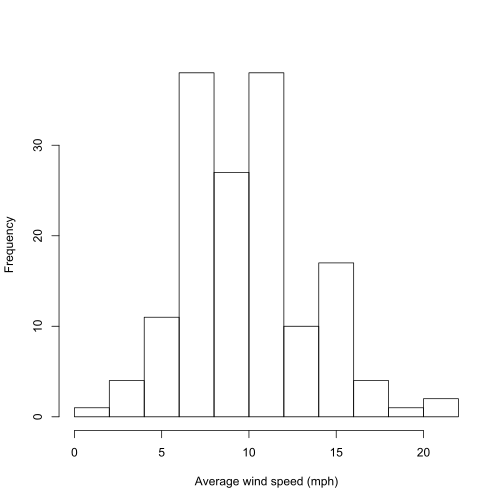
\includegraphics[width=0.8\textwidth,alt={a histogram}]{figures/SimpleGraphsHistAirQualityWind2-1} 

\SVGLink{SimpleGraphsHistAirQualityWind2} 
% filename SimpleGraphs011.Rnw 

\end{center} 
\end{exhibit} 
 
Variable names should be informative but aren't always what we want to see in graphs. Notice that in Exhibit~\ref{AirQualityHistWind2}, I've made the x-axis label more informative by indicating the units of measurement for the wind speed. As I already have a caption for my Exhibit, I have chosen to remove the default title by adding the argument \code{main=""} to the \Rcmd{hist} command. 
 
Aside from the alteration of the default axis label and the change in the main title for our histograms, we could make quite a number of changes. The \Rcmd{hist} function allows the user various options for the way the bars are filled in for example. It's often worth checking the default behaviour and then seeing if the resulting graph is what you want. If it isn't, then investigate your options by looking at the relevant help file; in this case type \code{?hist} to get to the help for the \Rcmd{hist} function. 
 
 Other graphs we create will show points marked with small hollow circles; we may wish to make these circles smaller, joined by line segments, filled in, a different colour or combinations of all of these attributes. The \Rcmd{par} function should be investigated to find out what is possible. Most graph functions allow the user the option of adding arguments that will be passed directly to the \Rcmd{par} function to obtain the same behaviour. Investigate the graphical parameters at some stage using \code{?par} but be warned, there are lots of adjustments that can be made. Experimenting is really the only option when it comes time to get your graph looking perfect. 
 
Additional text and/or lines can be added to some graph types. It may prove useful to show the line of best fit along with the data (illustrated in Chapter~\ref{Regression}) for example. We'll see how to do the fancy things in Chapter~\ref{ComplexGraphs}. 
 
\section{Other univariate summary graphs} 
 
Histograms aren't the ``be all and end all" for univariate summary graphs. As a case in point, they aren't at all useful for small sample sizes. Various other graphs appear in introductory statistics courses and that is why they appear here. I don't mean to support one over another at all --- that's up to you to determine. 
 
\subsection{Boxplots} 
 
Boxplots show us quickly the shape of the distribution of a sample. They show the median, lower and upper quartiles, and the minimum and maximum of a sample. They will also identify points as outliers if these points are too far from the bulk of values in the sample. 
 
Exhibit~\ref{AirQualityBoxplot} shows us the boxplot for the average wind speed at LaGuardia airport. Notice that I have added an additional command to set up the size of the graph window. The \Rcmd{windows} command has various aliases --- \Rcmd{x11}, \Rcmd{X11}, \Rcmd{win.graph} --- none of which are required if the standard width and height of the graph window are acceptable. You may wish to see why I've changed the height of the graph window by ignoring the \Rcmd{windows} command from Exhibit~\ref{AirQualityBoxplot} 
 
\begin{exhibit} 
\begin{center} 
\caption{Boxplot of Average wind speed in miles per hour at 0700 and 1000 hours at LaGuardia Airport. Obtained from the \Robject{air quality} data set.} 
\label{AirQualityBoxplot} 
% filename SimpleGraphs012.Rnw 

\begin{Schunk}
\begin{Sinput}
> ## windows(7, 5)
> boxplot(Wind, horizontal=TRUE, xlab="Wind speed (mph)")
\end{Sinput}
\end{Schunk}
\includegraphics[width=0.8\textwidth,alt={a boxplot}]{figures/SimpleGraphsBoxplotAirQualityWind-1} 

\SVGLink{SimpleGraphsBoxplotAirQualityWind} 

% filename SimpleGraphs013.Rnw 

\end{center} 
\end{exhibit} 
 
Notice that I've changed the default orientation of the boxplot by adding the argument \code{horizontal=TRUE} to the \Rcmd{boxplot} command. I have also ensured the more informative axis label for wind speed is included using the \Rarg{xlab} argument in the command. 
 
\subsection{Comparative boxplots} 
 
Boxplots are often useful for comparing several small samples at once. We must ensure that the same axis is used for the units of measure of interest and the easiest way to ensure this is to put the various samples into the same graphic with only one axis rather than having a series of single boxplots each having their own axis. 
 
For the purposes of illustration, I want to show the distribution of the daily average wind speeds for the five months separately.  
\begin{exhibit} 
\begin{center} 
\caption{Comparative boxplots for the Average wind speed in miles per hour at 0700 and 1000 hours at LaGuardia Airport separated into groups for the months of May to September 1973. Data was Obtained from the \Robject{air quality} data set.} 
\label{AirQualityCompBoxplotWindMonth} 
% filename SimpleGraphs014.Rnw 

\begin{Schunk}
\begin{Sinput}
> boxplot(Wind~Month, xlab="Month", ylab="Wind speed (mph)") 
\end{Sinput}
\end{Schunk}
\includegraphics[width=0.8\textwidth,alt={a comparative boxplot}]{figures/SimpleGraphsCompBoxplotAirQualityWind-1} 



\SVGLink{SimpleGraphsCompBoxplotAirQualityWind} 

% filename SimpleGraphs015.Rnw 

\end{center} 
\end{exhibit} 
The comparative boxplot is created using a formula to describe the relationship between the two variables that are referred to in our graph. The use of the tilde symbol between \Robject{Wind} and \Robject{Month} could be read as something like ``average wind speed depends on the month" --- well a theory that might be illustrated in our graph anyway. Certainly it is the potential for this relationship to exist that may be exposed through use of the comparative boxplot. 
 
\subsection{Dotplots} 
 
Dotplots aren't everyone's cup of tea but they are frequently offered as substitutes for boxplots and histograms. Again, I chose to alter the default window size for the example given in Exhibit~\ref{AirQualityDotPlotWind} 
because I didn't like the way the regular graph window presented this graph. 
\begin{exhibit} 
\begin{center} 
\caption{Dotplot of the Average wind speed in miles per hour at 0700 and 1000 hours at LaGuardia Airport. Obtained from the \Robject{air quality} data set.} 
\label{AirQualityDotPlotWind} 
% filename SimpleGraphs016.Rnw 

\begin{Schunk}

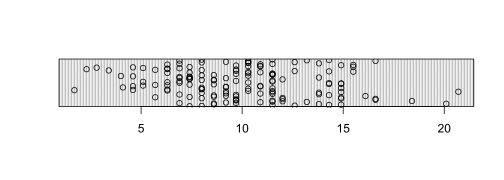
\includegraphics[width=0.8\textwidth]{figures/SimpleGraphsDotPlot-1} \end{Schunk}
% filename SimpleGraphs017.Rnw 

\end{center} 
\end{exhibit} 
 
Some people find the standard dotplot that \R{} creates a little artificial. The spacing between points horizontally and vertically is captured by the human eye, but this graph is a single dimensional representation. Adding jitter to the data allows points where there are ties to be represented by a pair of points on the graph rather than two perfectly overlaid points which look like a single point. The \Rcmd{jitter} command can be embedded within the command for creation of a dotplot, but is not required for our example data as there are no ties. If there were a large number of ties, we would have used the command \code{dotchart(jitter(Wind))}. 
 
 
 
\subsection{Simple line plots} 
 
Occasionally it's useful to see how a measurement changes over the time data were collected. \R{} does this very simply using the \Rcmd{plot} command as shown in Exhibit~\ref{AirQualityLinePlotTemp} which is for the maximum daily air temperatures at LaGuardia airport from 1 May to 30 September 1973. We can see periods of time where the maximum temperatures were fairly consistent and periods where it was fairly volatile. The middle of the graph is for the month of July which is the height of summer in New York and as a consequence we expect to see few points nearer the lower part of the graph during this period. 
\begin{exhibit} 
\begin{center} 
\caption{Line plot of the maximum daily temperatures from 1 May to 30 September 1973, measured in degrees Fahrenheit, at LaGuardia Airport. Data were obtained from the \Robject{air quality} data set.} 
\label{AirQualityLinePlotTemp} 
% filename SimpleGraphs018.Rnw 

\begin{Schunk}
\begin{Sinput}
> plot(Temp, ylim=c(50,100)) 
\end{Sinput}

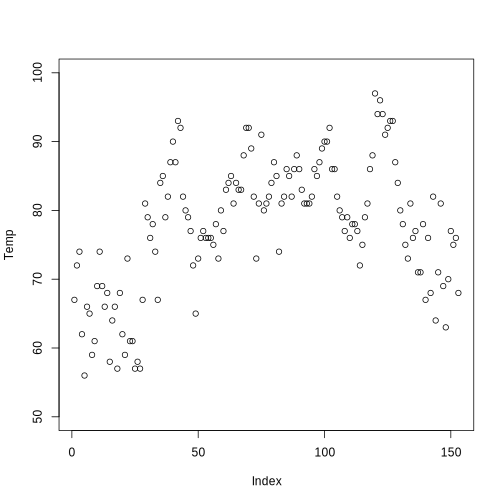
\includegraphics[width=0.8\textwidth]{figures/SimpleGraphsLinePlot-1} \end{Schunk}
% filename SimpleGraphs019.Rnw 

\end{center} 
\end{exhibit} 
\begin{exhibit} 
\begin{center} 
\caption{Line plot of the maximum daily temperatures from 1 May to 30 September 1973, measured in degrees Fahrenheit, at LaGuardia Airport. Data were obtained from the \Robject{air quality} data set.} 
\label{AirQualityLinePlotTemp2} 
% filename SimpleGraphs020.Rnw 

\begin{Schunk}
\begin{Sinput}
> plot(Temp, ylim=c(50,100), type="l") 
\end{Sinput}

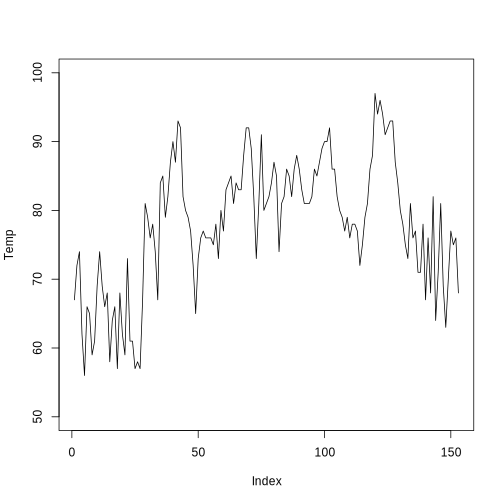
\includegraphics[width=0.8\textwidth]{figures/SimpleGraphsLinePlot2-1} \end{Schunk}
% filename SimpleGraphs021.Rnw 

\end{center} 
\end{exhibit} 
 
%%default is points and lines are wanted. explain 
 
Notice that we have altered the range of values covered by the $y$-axis using a specific command. The \Rarg{ylim} has a corresponding \Rarg{xlim} to create limits for the $x$-axis. Adding one more argument to the \Rcmd{plot} command will change the plotting from points to lines (shown in Exhibit~\ref{AirQualityLinePlotTemp2}). Combinations of points and lines can be obtained (not shown); the user can also alter the style of the points and lines being printed. 
 
There is a simpler way to generate time series plots which we demonstrate in Chapter~\ref{TimeSeries}. It is easier to augment this line plot than the time series plot and in so doing, we will gain an insight into how other plots like the time series plot are created. 
 
 
\section{Quantile-quantile plots} 
 
The most common quantile-quantile plot we might wish to create is used to investigate the usefulness of the normal distribution to model a variable's distribution. Normal quantiles are created automatically for the normal quantile plot when it is generated using the \Rcmd{qqnorm} command. The default plot for this is shown in Exhibit~\ref{AirQualityNormPlotWind}. 
 
If these data were normally distributed, the points on the plot would lie on a straight line. The \Rcmd{qqline} command adds the straight line to the plot to assist with determining the linearity of the points. 
 
\begin{exhibit} 
\begin{center} 
\caption{Normal probability plot of the Average wind speed in miles per hour at 0700 and 1000 hours at LaGuardia Airport. Obtained from the \Robject{air quality} data set.} 
\label{AirQualityNormPlotWind} 
% filename SimpleGraphs022.Rnw 

\begin{Schunk}
\begin{Sinput}
> qqnorm(Wind) 
> qqline(Wind) 
\end{Sinput}

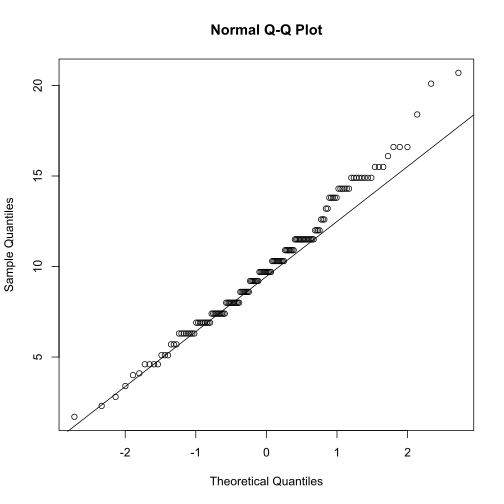
\includegraphics[width=0.8\textwidth]{figures/SimpleGraphsNormPlot-1} \end{Schunk}
% filename SimpleGraphs023.Rnw 

\end{center} 
\end{exhibit} 
 
\section{Scatter plots} 
 
Scatter plots are created using the \Rcmd{plot} command by one of two methods. Exhibit~\ref{AirQualityScatterTempWind} was created using 
% filename SimpleGraphs024.Rnw 

\begin{Schunk}
\begin{Sinput}
> plot(Wind, Temp) 
\end{Sinput}
\end{Schunk}
% filename SimpleGraphs025.Rnw 

but the same plot can be generated using what is known as a formula. In this case, only one argument is given to the \Rcmd{plot} command but both variables of interest are in that argument. 
% filename SimpleGraphs026.Rnw 

\begin{Schunk}
\begin{Sinput}
> plot(Temp~Wind) 
\end{Sinput}
\end{Schunk}
% filename SimpleGraphs027.Rnw 

The tilde symbol is often read as ``\ldots is distributed as\ldots" but we might simplify this to be read as ``follows". This makes some sense as we generally create a scatter plot to see if one variable follows the other; in this case we are seeing if temperature depends on wind speed in some way. 
 
\begin{exhibit} 
\begin{center} 
\caption{Scatter plot of the maximum daily temperature against the Average wind speed at 0700 and 1000 hours, both recorded at LaGuardia Airport. Data were obtained from the \Robject{air quality} data set.} 
\label{AirQualityScatterTempWind} 
% filename SimpleGraphs028.Rnw 

\begin{Schunk}
\begin{Sinput}
> plot(Wind, Temp) 
\end{Sinput}

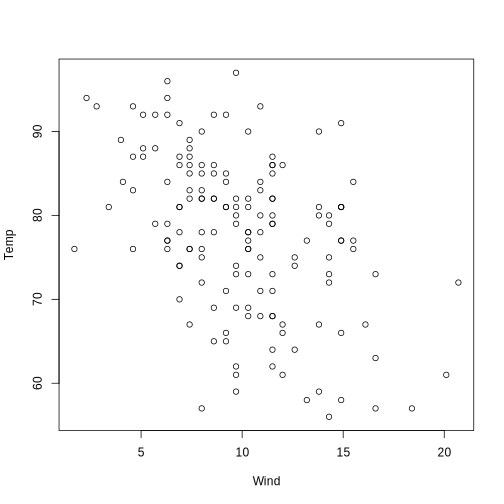
\includegraphics[width=0.8\textwidth]{figures/SimpleGraphsScatter-1} \end{Schunk}
% filename SimpleGraphs029.Rnw 

\end{center} 
\end{exhibit} 
 
\section{Scatter plot matrices} 
\label{ScatterPlotMatrices} 
 
A scatter plot matrix is just a matrix of scatter plots where each variable is plotted against all other variables. This graphic is therefore very useful for a preliminary look at multivariate data. In \R{}, we obtain this graphic using the \Rcmd{pairs} command as illustrated in Exhibit~\ref{AirQualityScatterPlotMatrix}. 
 
Only four of the variables within the \Robject{air quality} data have been used in this example because the variables for the month and day take discrete values and therefore do not suit scatter plots --- take a look for yourself if you must but it's probably better to think about why this is the case before you look at the graphs. To select the four variables of interest, I have created a \Rclass{data.frame} with the variables I want included,; this \Rcmd{data.frame} command is then nested within the \Rcmd{pairs} command. 
\begin{exhibit} 
\begin{center} 
\caption{A scatter plot matrix of the numeric variables within the \Robject{airquality} data set.} 
\label{AirQualityScatterPlotMatrix}. 
% filename SimpleGraphs030.Rnw 

\begin{Schunk}
\begin{Sinput}
> pairs(data.frame(Ozone, Solar.R, Wind, Temp)) 
\end{Sinput}

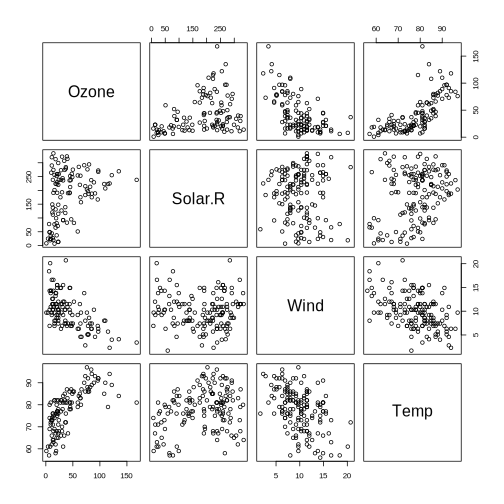
\includegraphics[width=0.8\textwidth]{figures/SimpleGraphsMatrixPlot-1} \end{Schunk}
% filename SimpleGraphs031.Rnw 

\end{center} 
\end{exhibit} 
 
Note that the names of the variables appear in the spaces on the leading diagonal and that the graphs on either side of the diagonal plot the same data but with the axes reversed. Sometimes the human eye will pick up a relationship when the data are presented one way better than the other way. 
 
\section{Graphs for discrete valued variables} 
 
\R{} does not contain many graphs for discrete valued variables. 
 
\subsection{Bar charts} 
\label{BarCharts} 
 
If a variable is considered by \R{} to be a \Rclass{factor}, then the default action of the \Rcmd{plot} command is to construct a bar chart. This is illustrated using a data set which is part of the default installation of \R{} called \Robject{state.region} examined using 
% filename SimpleGraphs032.Rnw 

\begin{Schunk}
\begin{Sinput}
> str(state.region) 
\end{Sinput}
\begin{Soutput}
 Factor w/ 4 levels "Northeast","South",..: 2 4 4 2 4 4 1 2 2 2 ...
\end{Soutput}
\begin{Sinput}
> levels(state.region) 
\end{Sinput}
\begin{Soutput}
[1] "Northeast"     "South"         "North Central"
[4] "West"         
\end{Soutput}
\end{Schunk}
% filename SimpleGraphs033.Rnw 

Given this variable is a \Rclass{factor} with four levels it is well suited to presentation in a bar chart, as seen in Exhibit~\ref{StateRegionBarChart}. 
 
\begin{exhibit} 
\begin{center} 
\caption{A bar chart showing which of the regions each of the fifty U.S. states belongs} 
\label{StateRegionBarChart} 
% filename SimpleGraphs034.Rnw 

\begin{Schunk}
\begin{Sinput}
> plot(state.region) 
\end{Sinput}

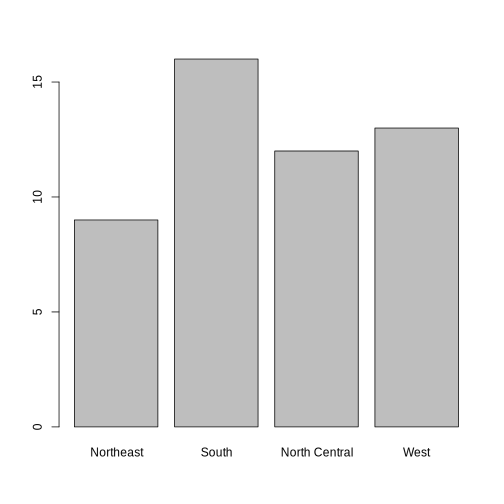
\includegraphics[width=0.8\textwidth]{figures/SimpleGraphsStateRegionBarChart-1} \end{Schunk}
% filename SimpleGraphs035.Rnw 

\end{center} 
\end{exhibit} 
 
This figure was created from the raw data, that is the regions for each of the fifty states in the U.S. If we had summary data with counts for each of the categories, we would need to use the \Rcmd{barplot} command. The \Rcmd{summary} command shows us how many states fall into each category in this instance. 
% filename SimpleGraphs036.Rnw 

\begin{Schunk}
\begin{Sinput}
> summary(state.region) 
\end{Sinput}
\begin{Soutput}
    Northeast         South North Central          West 
            9            16            12            13 
\end{Soutput}
\end{Schunk}
% filename SimpleGraphs037.Rnw 

These values are then plotted in Exhibit~\ref{StateRegionBarChart2}. 
\begin{exhibit} 
\begin{center} 
\caption{A bar chart showing which of the regions each of the fifty U.S. states belongs} 
\label{StateRegionBarChart2} 
% filename SimpleGraphs038.Rnw 

\begin{Schunk}
\begin{Sinput}
> barplot(summary(state.region)) 
\end{Sinput}

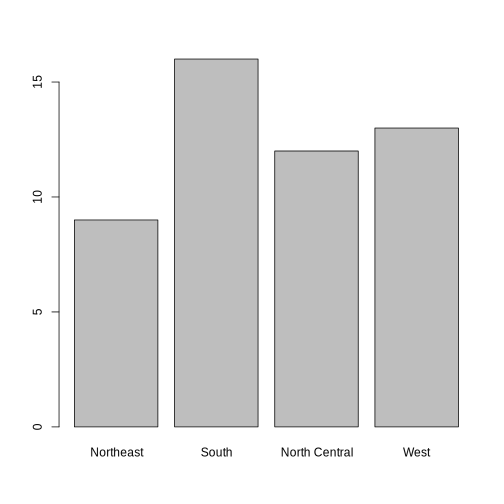
\includegraphics[width=0.8\textwidth]{figures/SimpleGraphsStateRegionBarChart2-1} \end{Schunk}
% filename SimpleGraphs039.Rnw 

\end{center} 
\end{exhibit} 
 
While this data set is rather trivial, it is useful for demonstrating one more feature. Note that both in the output above and in Exhibit~\ref{StateRegionBarChart}, the Western region is the last category. To reorder the regions in the bar chart is actually fairly straight forward. All we need to do is make a small addition to the existing commands. 
% filename SimpleGraphs040.Rnw 

\begin{Schunk}
\begin{Sinput}
> summary(state.region)[c(4,2,3,1)] 
\end{Sinput}
\begin{Soutput}
         West         South North Central     Northeast 
           13            16            12             9 
\end{Soutput}
\end{Schunk}
% filename SimpleGraphs041.Rnw 

and re-create the bar chart accordingly (see Exhibit~\ref{StateRegionBarChartImp}). 
\begin{exhibit} 
\begin{center} 
\caption{An improved bar chart showing which of the regions each of the fifty U.S. states belongs} 
\label{StateRegionBarChartImp} 
% filename SimpleGraphs042.Rnw 

\begin{Schunk}
\begin{Sinput}
> barplot(summary(state.region)[c(4,2,3,1)]) 
\end{Sinput}

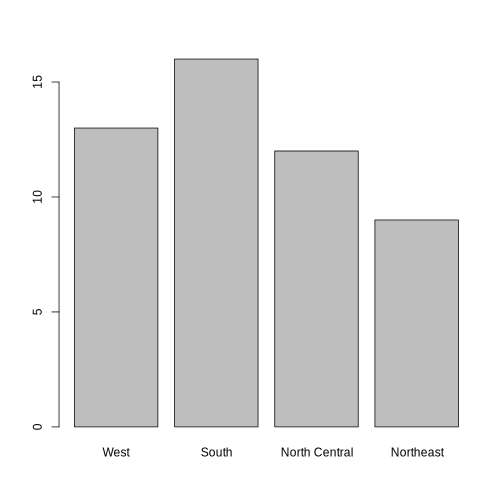
\includegraphics[width=0.8\textwidth]{figures/SimpleGraphsStateRegionBarChartImp-1} \end{Schunk}
% filename SimpleGraphs043.Rnw 

\end{center} 
\end{exhibit} 
 
\subsection{Pie charts} 
 
OK, if you must do so, make a pie chart using the \Rcmd{pie} command. Even the help for this command says they are a bad representation for data, stating ``Pie charts are a very bad way of displaying information. The eye is good at judging linear measures and bad at judging relative areas. A bar chart or dot chart is a preferable way of displaying this type of data."  
 
The pie chart for the \Robject{state.region} data is given in Exhibit~\ref{StateRegionPieChart}. 
\begin{exhibit} 
\begin{center} 
\caption{A pie chart showing which of the regions each of the fifty U.S. states belongs} 
\label{StateRegionPieChart} 
% filename SimpleGraphs044.Rnw 

\begin{Schunk}
\begin{Sinput}
> pie(summary(state.region)) 
\end{Sinput}

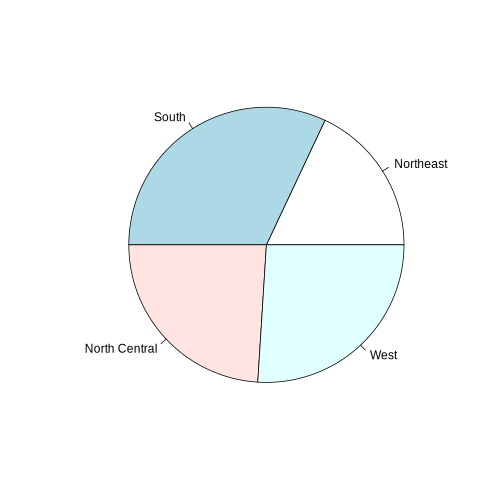
\includegraphics[width=0.8\textwidth]{figures/SimpleGraphsStateRegionPieChart-1} \end{Schunk}
% filename SimpleGraphs045.Rnw 

\end{center} 
\end{exhibit} 
 
 
\section{Closing} 
 
If you are carrying on working with \R{} you might wish to remove direct access to the data sets we used in this chapter by issuing the following commands 
% filename DetachAirQuality.Rnw 

\begin{Schunk}
\begin{Sinput}
> detach(airquality) 
\end{Sinput}
\end{Schunk}
% filename CleanUp.Rnw 



